% !Mode:: "TeX:UTF-8" 
% !TEX program = xelatex
\documentclass [t,12pt,mathserif] {beamer} 

\usepackage[english]{babel}
\usepackage[utf8]{inputenc}
\usepackage[T1]{fontenc}
\usepackage{csquotes}
\usepackage{expl3,biblatex}
\usepackage{booktabs}
\usepackage{color,xcolor}
\usepackage{graphicx,caption,wrapfig,setspace}
\usepackage{amsthm,thmtools,amsmath,amsfonts,amssymb,dsfont} 
\usepackage{soul}
\usepackage{xeCJK}
\usepackage{newtxtext, newtxmath}

\usetheme{Madrid}
\usecolortheme{crane}
% set font
\usefonttheme{serif}

\definecolor{titlecolor}{RGB}{227, 169, 5}

\addtobeamertemplate{block begin}{%
  \setlength{\textwidth}{0.9\textwidth}%
}{}

\addtobeamertemplate{block alerted begin}{%
  \setlength{\textwidth}{0.9\textwidth}%
}{}

\addtobeamertemplate{block example begin}{%
  \setlength{\textwidth}{0.9\textwidth}%
}{}


\makeatletter
\let\HL\hl
\renewcommand\hl{%
  \let\set@color\beamerorig@set@color
  \let\reset@color\beamerorig@reset@color
  \HL}
\makeatother


\addbibresource{bibliography.bib}

% \usefonttheme[onlymath]{serif}
\mathversion{bold}
\setbeamerfont{normal text}{family=\sffamily,series=\mdseries}
\setbeamerfont{alerted text}{series=\bfseries}
\setbeamerfont{frametitle}{series=\bfseries}
\AtBeginDocument{\usebeamerfont{normal text}}

\renewcommand\baselinestretch{1.5}
\renewcommand\arraystretch{1.3}
\allowdisplaybreaks
\everymath{\displaystyle}

\beamertemplatenavigationsymbolsempty
\setbeamertemplate{footline}[page number]{} 
 \addtobeamertemplate{frametitle}{\vspace*{-0.5em}}{}
 

\newtheoremstyle{mydef}%
{3pt}{3pt}{\bfseries}{}{\bfseries\color{red}}{}{.5em}{}
\theoremstyle{mydef}
\newtheorem{dfn}{定义}
\newtheorem{thm}{定理}[section] 

\newtheoremstyle{myliti}%
{3pt}{3pt}{\bfseries}{}{\bfseries\color{blue}}{}{.5em}{}
\theoremstyle{myliti}
\newtheorem{ex}{例}

\newtheoremstyle{mystarli}%
{3pt}{3pt}{\bfseries}{}{\bfseries\color{blue}}{}{.5em}{}
\theoremstyle{mystarli}
\newtheorem{starli}{*例}

\setbeamertemplate{theorems}[numbered]
\setbeamertemplate{caption}[numbered]

\newcommand{\liang}[1]{\textcolor{blue}{#1}}
\newcommand{\tuchu}[1]{\textcolor{red}{#1}}
\setbeamertemplate{blocks}[rounded][shadow=false]

\newcommand{\blue}{\textcolor{blue}}
\newcommand{\red}{\textcolor{red}}
\newcommand{\magenta}{\textcolor{magenta}}
\newcommand{\teal}{\textcolor{teal}}
% \newcommand{\bena}{\vspace{-0.7\baselineskip}\begin{eqnarray}\begin{array}{l}}
% \newcommand{\eena}{\end{array}\end{eqnarray}\vskip -0.3\baselineskip}
% \newcommand{\benas}{\vspace{-0.7\baselineskip}\begin{eqnarray*}\begin{array}{l}}
% \newcommand{\eenas}{\end{array}\end{eqnarray*}\vskip -0.6\baselineskip}
\newcommand{\bena}{\begin{eqnarray}\begin{array}{l}}
\newcommand{\eena}{\end{array}\end{eqnarray}}
\newcommand{\benas}{\begin{eqnarray*}\begin{array}{l}}
\newcommand{\eenas}{\end{array}\end{eqnarray*}}
\newcommand{\ben}{\begin{eqnarray}}
\newcommand{\een}{\end{eqnarray}}
\newcommand{\bea}{\begin{array}}
\newcommand{\eea}{\end{array}}
\newcommand{\beq}{\begin{equation}}
\newcommand{\eeq}{\end{equation}}
\newcommand{\bec}{\setstretch{1.3}\begin{cases}}
\newcommand{\eec}{\end{cases}}
\newcommand{\beu}{\begin{enumerate}}
\newcommand{\eeu}{\end{enumerate}}
\def\rd{\ensuremath{ \mathrm{~d} }}
\def\re{\ensuremath{ \mathrm{e} }}
\def\vsp{\vskip 0.3\baselineskip}
\newcommand{\zhu}[1]{
\begin{alertblock}{}
 \textcolor{blue}{注 } #1
        \par  
\end{alertblock}
}
\def\jie{\textcolor{blue}{解} }
\def\zheng{\textcolor{blue}{证} }

\makeatletter
\setbeamertemplate{theorem begin}
{%  
\begin{\inserttheoremblockenv}
  {}{
%   \usebeamerfont*{block title}
  \usebeamercolor[fg]{block title}%
  \inserttheoremheadfont
  \inserttheoremname
  \inserttheoremnumber
  \ifx \inserttheoremaddition \empty \else\ \inserttheoremaddition\fi
%   \inserttheorempunctuation
  }
%   \normalfont
  }
  \setbeamertemplate{theorem end}{\end{\inserttheoremblockenv}}
\makeatother

% \declaretheoremstyle[
%     headfont=\normalfont
% ]{definition}

\AtBeginDocument{%
  \addtolength\abovedisplayskip{-0.5\baselineskip}%
  \addtolength\belowdisplayskip{-0.5\baselineskip}%
} 

\setbeamercolor{alerted text}{fg=titlecolor!70!blue}

% \setbeamercolor{titlelike}{fg=titlecolor}

\setbeamerfont{titlelike}{family=\sffamily,series=\bfseries}

\setbeamerfont{section number projected}{%
  family=\rmfamily,series=\bfseries,size=\normalsize}
\setbeamercolor{section number projected}{bg=titlecolor!50!red,fg=white}
\setbeamerfont{section in toc}{family=\sffamily,series=\bfseries,size=\normalsize}
\setbeamerfont{section in toc shaded}{size=\normalsize}

\setbeamerfont{title}{family=\sffamily,series=\bfseries,size=\LARGE}

\title[数列极限]{数列极限}
\institute[]{天津师范大学,数学科学学院}
% \titlegraphic{\includegraphics[height=2.0cm]{imologo.png}}
\author[Jun Li]{
	李~君 }
\date{2023年6月}


\begin{document}
\begin{frame}
\maketitle
\end{frame}

\begin{frame}
\frametitle{目~~录}
\setcounter{tocdepth}{2}
\tableofcontents
\end{frame}


%%%%%%%%%%%%%%%%%%%%%%%%%%%%%%%%%%%%%
\setcounter{section}{1}
\section{第二章~~数列极限}
\subsection{数列极限的概念}
\begin{frame}{$\S 1$ 数列极限的概念}
 \alert{数列极限是整个数学分析最重要的基础 之一, 它不仅与函数极限密切相关, 而且 为今后学习级数理论提供了极为丰富的准 备知识。}\\
~\\
一、数列的定义\\
二、一个经典的例于\\
三、收敛数列的定义\\
四、按定义验证极限\\
五、再论“ $\varepsilon-N$ ”说法、一些例子    
\end{frame}

\begin{frame}{一、数列的定义}

若函数 $\boldsymbol{f}$ 的定义域为全体正整数的集合 $\mathrm{N}_{+}$, 则称
\benas
f: \mathbf{N}_{+} \rightarrow \mathbf{R}$ 或 $f(n), n \in \mathbf{N}_{+}\eenas
为数列. 因为 $\mathbf{N}_{+}$的所有元素可以从小到大排列出来, 所以我们也将数列写成
\benas
a_1, a_2, \cdots, a_n, \cdots,
\eenas
或简记为 $\left\{a_n\right\}$. 这里 $a_n$ 称为数列 $\left\{a_n\right\}$ 的通项.
\begin{wrapfigure}{r}{0.45\textwidth}
\vspace{-0.85\baselineskip}
% \renewcommand{\figurename}{图}
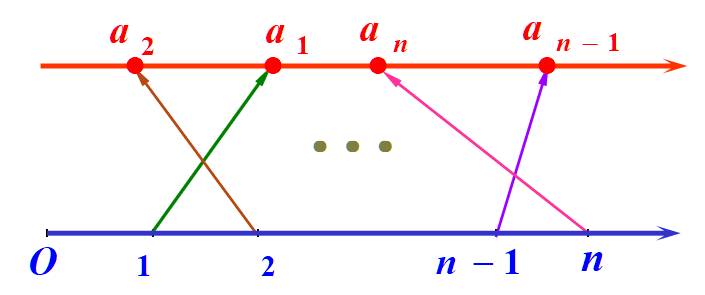
\includegraphics[width=0.4\textwidth]{figures/shuliedingyi1.png}
% \caption{~}
\vspace{-0.85\baselineskip}
\end{wrapfigure}

\end{frame}

\begin{frame}{二、一个经典的例子}
古代哲学家庄周所著的《庄子.天下篇》引用了 一句话:“一尺之棰, 日取其半,万世不竭”。它的 意思是:一根长为一尺的木棒, 每天截下一半, 这 样的过程可以无限制地进行下去.\\
我们把每天截下部分 (或剩下部分) 的长度列出:\\ 第一天截下 $\frac{1}{\mathbf{2}}$, 第二天截下 $\frac{1}{\mathbf{2}^2}, \cdots$, 第 $n$ 天截下 $\frac{1}{2^n}, \cdots \cdot$\\ 这样就得到一个数列:
$$
\frac{1}{2}, \frac{1}{2^2}, \cdots, \frac{1}{2^n}, \cdots, \text { 或 }\left\{\frac{1}{2^n}\right\} .
$$
容易看出:数列 $\left\{\frac{1}{2^n}\right\}$ 的通项 $\frac{1}{2^n}$ 随着 $n$ 的无限增 大而无限趋于 $0$ .
    
\end{frame}

\begin{frame}{  三、收敛数列的定义}%%%%%%%

一般地说, 对于数列 $\left\{a_n\right\}$, 若当 $n$ 充分变大时, $a_n$ 能无限地接近某个常数 $\boldsymbol{a}$, 则称 $\left\{a_n\right\}$ 收敛于 $\boldsymbol{a}$. 下面给出严格的数学定义.
\begin{dfn}
设 $\left\{a_n\right\}$ 为一个数列, $a$ 为一个常数, 若对于 任意的正数 $\varepsilon>0$, 总存在正整数 $N$, 使当 $n>N$ 时,
\benas
\left|a_n-a\right|<\varepsilon,
\eenas
则称数列 $\left\{a_n\right\}$ 收敛于 $a$, 又称 $a$ 为数列 $\left\{a_n\right\}$ 的极限, 记作
\benas
\lim _{n \rightarrow \infty} a_n=a. \quad  (\text{或 } \quad a_n \rightarrow a,~ n \rightarrow \infty)
\eenas
\end{dfn} 


\end{frame}

\begin{frame}{}%%%%%%
  若 $\left\{a_n\right\}$ 不收敛, 则称 $\left\{a_n\right\}$ 为发散数列.
  \begin{wrapfigure}{l}{0.6\textwidth}
\vspace{-0.85\baselineskip}
% \renewcommand{\figurename}{图}
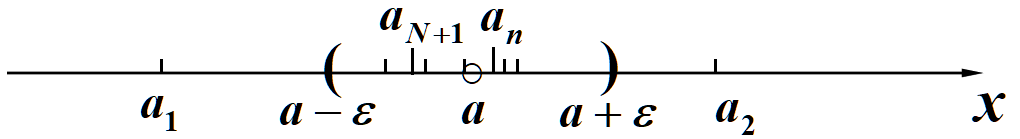
\includegraphics[width=0.6\textwidth]{figures/shuzhoushulie1.png}
% \caption{~}
% \vspace{-0.5\baselineskip}
\end{wrapfigure}
\\~\\
  \begin{alertblock}{}
 \liang{注} 定义 1 这种陈述方式, 俗称为 \liang{`` $\varepsilon-N$ "说法}.     
  \end{alertblock}{}

 
\end{frame}

\begin{frame}{ 四、按定义验证极限}%%%%
为了加深对数列收敛定义的了解, 下面结合例题加 以说明, 希望大家对 “ $\varepsilon-N$ ”说法能有正确的认识. \\
\begin{ex}
用定义验证: $\lim _{n \rightarrow \infty} \frac{1}{n}=0$.
\end{ex}
\liang{分析} 对于任意正数 $\varepsilon$, 要使 $\left|\frac{1}{n}-0\right|<\varepsilon$, 只要 $n>\frac{1}{\varepsilon}$.\\
\zheng 对于任意的正数 $\varepsilon$, 取 $N=\left[\frac{1}{\varepsilon}\right]$, 当 $n>N$ 时, $\left|\frac{1}{n}-0\right|<\varepsilon$, 所以 $\lim _{n \rightarrow \infty} \frac{1}{n}=0$.  
\end{frame}

\begin{frame}{}%%%%
\begin{ex}
用定义验证 $\lim _{n \rightarrow \infty} q^n=0 \quad(0<|q|<1)$.
\end{ex} 
\liang{分析} 对于任意的正数 $\varepsilon$, 要使 $\left|q^n-0\right|<\varepsilon$, 只要
$$
n>\frac{\log \varepsilon}{\log |q|} . 
$$
\zheng $\forall \varepsilon>0$ (不妨设 $0<\varepsilon<1$ ), 取 $N=\left[\frac{\log \varepsilon}{\log |q|}\right]+1$, 当 $n>N$ 时,有
$$
\left|\boldsymbol{q}^n-\mathbf{0}\right|<\boldsymbol{\varepsilon}
$$
这就证明了 $\lim _{n \rightarrow \infty} q^n=0$.
    
\end{frame}


\begin{frame}{}%%%%
\begin{ex}
用定义验证 $\lim _{n \rightarrow \infty} \frac{n^2}{3 n^2-n-7}=\frac{1}{3}$.
\end{ex} 
\liang{分析} 任给 $\varepsilon>0$, 由
$$
\left|\frac{n^2}{3 n^2-n-7}-\frac{1}{3}\right|=\left|\frac{n+7}{3\left(3 n^2-n-7\right)}\right|,
$$
当 $n \geq 7$ 时, $n+7 \leq 2 n, 3 n^2-n-7 \geq 3 n^2-2 n \geq 2 n^2$,
故要使 $\left|\frac{n+7}{3\left(3 n^2-n-7\right)}\right| \leq \frac{2 n}{6 n^2}=\frac{1}{3 n}<\varepsilon $ 成立, 只要 $n>\frac{1}{3 \varepsilon}$ 即可.  \\
~\\
\liang{注意} 解这个不等式是在 $n \geq 7$ 的条件下进行的. 
\end{frame}


\begin{frame}{}%%%%
\zheng 对于任意的正数 $\varepsilon$, 取
$$
N=\max \left\{7,\left[\frac{1}{3 \varepsilon}\right]+1\right\} , 
$$
当 $n>N$ 时, 有
$$
\left|\frac{n^2}{3 n^2-n-7}-\frac{1}{3}\right|<\varepsilon,
$$
即得
$$
\lim _{n \rightarrow \infty} \frac{n^2}{3 n^2-n-7}=\frac{1}{3} .
$$   
\end{frame}


\begin{frame}{}%%%%
\begin{ex}
 用定义验证 $\lim _{n \rightarrow \infty} \sqrt[n]{a}=1$, 其中 $a>0$. 
\end{ex}
\zheng 这里只验证 $a>1$ 的情形 $(0<a<1$ 时自证 $)$. 设 $\alpha_n=a^{\frac{1}{n}}-1$. 因为 $a=\left(1+\alpha_n\right)^n \geq 1+n \alpha_n$, 所以
$$
0<\alpha_n=\sqrt[n]{a}-1 \leq \frac{a-1}{n} .
$$
故对于任意正数 $\varepsilon$, 取 $N=\left[\frac{a-1}{\varepsilon}\right]+1$, 当 $n>N$ 时,
$$
|\sqrt[n]{a}-1|<\varepsilon.
$$
因此证得 $\lim _{n \rightarrow \infty} \sqrt[n]{a}=1$.  
\end{frame}



\begin{frame}{  五、再论`` $\varepsilon-N$ ”说法}%%%%
 从定义及上面的例题我们可以看出:\\
\liang{1. $\varepsilon$ 的任意性:} 定义中的 $\varepsilon$ 用来刻画数列 $\left\{a_n\right\}$ 的通 项与定数 $a$ 的接近程度. 显然正数 $\varepsilon$ 愈小,表示 $a_n$ 与 $a$ 接近的程度愈高; $\varepsilon$ 是任意的, 这就表示 $a_n$ 与 $\boldsymbol{a}$ 可以任意接近. 要注意, $\varepsilon$ 一旦给出, 在接下 来计算 $N$ 的过程中, 它暂时看作是确定不变的. 此外, 又因 $\varepsilon$ 是任意正数, 所以 $2 \varepsilon, 3 \varepsilon, \frac{\varepsilon}{2}, \cdots$ 等均可看作任意正数, 故定义 1 中的不等式
$$
\left|a_n-a\right|<\varepsilon
$$
可以用 $\left|a_n-a\right|<K \varepsilon$ ( $K$ 为某一正常数) 来代替. 
 
\end{frame}


\begin{frame}{}%%%%
再有, 我们还可以限定 $\varepsilon$ 小于某一个正数 ( 比如 $\varepsilon<1$ ). 事实上, 对 $0<\varepsilon<1$ 若能验证 $\left\{a_n\right\}$ 满足 定义 1 , 那么对 $\varepsilon \geq 1$ 自然也可以验证成立.\\
\liang{2. $N$ 的相对性:} 从定义 1 中又可看出, 随着 $\varepsilon$ 的取值 不同, $\boldsymbol{N}$ 当然也会不同. 但这并不意味着 $\boldsymbol{N}$ 是由$\varepsilon$ 惟一确定. 例如, 当 $n>N$ 时, 有
$$
\left|a_n-a\right|<\varepsilon,
$$
则当 $n>N_1=2 N$ 时, 对于同样的 $\varepsilon$, 更应有
$$
\left|a_n-a\right|<\varepsilon .
$$
也就是说, 在这里只是强调 $N$ 的存在性, 而不追 求 $N$ 的 “最佳性”.     
\end{frame}


\begin{frame}{}%%%%
\liang{ 3. 极限的几何意义}\\
从几何上看, “ $n>N$ 时有 $\left|a_n-a\right|<\varepsilon$ ”, 实际上就是 所有下标大于 $N$ 的 $a_n$ 全都落在邻域 $U(a ; \varepsilon)$ 之内, 而在 $U(a ; \varepsilon)$ 之外, $\left\{a_n\right\}$ 至多只有有限项( $N$ 项 ). 反过来, 如果对于任意正数 $\varepsilon$, 落在 $\boldsymbol{U}(a ; \varepsilon)$ 之外至 多只有有限项, 设这些项的最大下标为 $N$, 这就表 示当 $n>N$ 时, $a_n \in U(a ; \varepsilon)$, 即 $\lim _{n \rightarrow \infty} a_n=a$.  \\
以上是定义 1 的等价说法, 写成定义就是:\\
\begin{block}{} 
\tuchu{定义 $1^{\prime}$} 任给 $\varepsilon>0$, 若在 $U(a ; \varepsilon)$ 之外至多只有 $\left\{a_n\right\}$ 的有限多项, 则称数列 $\left\{a_n\right\}$ 收敛于 $a$. 这样, $\left\{a_n\right\}$ 不以 $a$ 为极限的定义也可陈述为:存在 $\varepsilon_0>0$, 使得在 $\left(a-\varepsilon_0, a+\varepsilon_0\right)$ 之外含有 $\left\{a_n\right\}$ 中的无限多 项.
\end{block}

\end{frame}


\begin{frame}{}%%%%
 \begin{alertblock}{}
\liang{注} $\left\{a_n\right\}$ 无极限 (即发散) 的等价定义为: $\left\{a_n\right\}$ 不以任何实数 $\boldsymbol{a}$ 为极限.  
 \end{alertblock}  

\end{frame}


\begin{frame}{4. 无穷小数列和无穷大数列}%%%%
\begin{dfn}
若 $\lim _{n \rightarrow \infty} a_n=0$, 则称 $\left\{a_n\right\}$ 为无穷小数列.
\end{dfn}    
\liang{例如} $\left\{\frac{1}{n^2}\right\}$ 和 $\left\{\frac{n !}{n^n}\right\}$ 是无穷小数列. 当 $|q|<1$ 时, $\left\{q^n\right\}$ 是无穷小数列.\\
以下定理显然成立,请读者自证.\\
\begin{thm}
数列 $\left\{a_n\right\}$ 收敛于 $a$ 的充要条件是: $\left\{a_n-a\right\}$ 是无穷小数列.
\end{thm} 
\end{frame}


\begin{frame}{}%%%%
\begin{dfn}
设 $\left\{a_n\right\}$ 是一数列, 若对任意 $G>0$, 总存在正 整数 $N$, 使得任意 $n>N,\left|a_n\right|>G$, 则称 $\left\{a_n\right\}$ 是\liang{无穷大数列}, 记作
$$
\lim _{n \rightarrow \infty} a_n=\infty \text {. }
$$
若 $\left|a_n\right|>G$, 改为 $a_n>G$ 或 $a_n<-G$, 则称 $\left\{a_n\right\}$ 是\liang{正无 穷大数列}或\liang{负无穷大数列}, 分别记作
$$
\lim _{n \rightarrow \infty} a_n=+\infty \text { 或 } \lim _{n \rightarrow \infty} a_n=-\infty . 
$$  
\end{dfn}  
\end{frame}

\begin{frame}{ 六、一些例子}%%%%
 
为了更好地理解 “ $\varepsilon-N$ ” 定义, 再举一些例题.
\begin{ex}
证明 $\left\{(-1)^n\right\}$ 发散.
\end{ex} 
\zheng 对于任意实数 $a$, 取 $\varepsilon_0=\frac{1}{2},\left\{a_n\right\}=\left\{(-1)^n\right\}$ 满足: 当 $a \leq 0(a \geq 0)$ 时, 在 $\left(a-\frac{\mathbf{1}}{\mathbf{2}}, a+\frac{\mathbf{1}}{\mathbf{2}}\right)$ 之外有无限多 个偶数项 (奇数项). 所以由定义 $1^{\prime},\left\{a_n\right\}$ 不以 $a$ 为极限. 又因 $\boldsymbol{a}$ 是任意的, 所以 $\left\{a_n\right\}$ 发散.  
\end{frame}


\begin{frame}{}%%%%
\begin{ex}
证明 $\lim _{n \rightarrow \infty} \frac{a^n}{n !}=0$.
\end{ex} 
\zheng $|a|>1$ 时, $\forall \varepsilon>0$, 取 $N=\frac{|a|^{[a \mid]+1}}{\varepsilon[|a|] \text { ! }}$, 当 $n>N$ 时,
$$
\left|\frac{a^n}{n !}-0\right|=\frac{\overbrace{|a| \cdots|a|}^{[|a|]} \overbrace{|a| \cdots|a|}^{n-[|a|]} }{1 \cdot 2 \cdots[|a|][|a|+1] \cdots n} \leq \frac{|a|^{[|a|]}}{[|a|] !} \cdot \frac{|a|}{n}<\varepsilon .
$$
当 $0<|a| \leq 1$ 时, 取 $N=\frac{1}{\varepsilon}, n>N$ 时, $\left|\frac{a^n}{n !}\right| \leq \frac{1}{n}<\varepsilon$, 从而 $\lim _{n \rightarrow \infty} \frac{a^n}{n !}=0$.  
\begin{alertblock}{}
\liang{注}  这里我们将 $\boldsymbol{N}$ 取为正数, 而非正整数. 实际上 $\boldsymbol{N}$ 只是表示某个时刻, 保证从这一时刻以后的所 有项都能使不等式 $\left|a_n-a\right|<\varepsilon$ 成立即可. 
\end{alertblock}
\end{frame}

\begin{frame}{}%%%%
\begin{ex}
 证明 $\lim _{n \rightarrow \infty} \sin \frac{1}{n}=0$. 
\end{ex}  
\zheng 我们用两种方法来证明.\\
(1) 任给正数 $\varepsilon$, 取 $N=\frac{1}{\varepsilon}$, 当 $n>N$ 时,
$$
\left|\sin \frac{1}{n}-0\right| \leq \frac{1}{n}<\varepsilon
$$
(2) 任给正数 $\varepsilon$, 限制 $\varepsilon<1$. 由
$$
\left|\sin \frac{1}{n}-0\right|=\sin \frac{1}{n}<\sin (\arcsin \varepsilon)=\varepsilon,
$$
可知只需取 $N=\frac{1}{\arcsin \varepsilon}$ 即可.
\begin{alertblock}{}
\liang{注}  这里假定 $0<\varepsilon<1$ 是必要的, 否则 $\arcsin \varepsilon$ 便 没有定义.
\end{alertblock}

\end{frame}


\begin{frame}{ 复习思考题}%%%%
1. 极限定义中的 $\forall \varepsilon, \exists N ”$ 是否可以写成 $\exists N$, $\forall \varepsilon$ "? 为什么?\\
2. $\lim _{n \rightarrow \infty} a_n=a \Rightarrow \lim _{n \rightarrow \infty}\left|a_n\right|=|a|$, 反之是否成立?\\
3. 已知 $\lim _{n \rightarrow \infty} a_n=A, \sigma: N \rightarrow N$ 是一个一一映射. 请依据极限定义证明: $\lim _{n \rightarrow \infty} a_{\sigma(n)}=A$.   
\end{frame}

\subsection{收敛数列的性质}

% \begin{frame}{Reference} %%%
% \nocite*
% \bibliographystyle{apalike}
% \bibliography{ref}
% \end{frame}

\end{document}


\begin{frame}{}%%%%
    
\end{frame}